\documentclass[12pt]{aghdpl}
% \documentclass[en,12pt]{aghdpl}  % praca w języku angielskim

% Lista wszystkich języków stanowiących języki pozycji bibliograficznych użytych w pracy.
% (Zgodnie z zasadami tworzenia bibliografii każda pozycja powinna zostać utworzona zgodnie z zasadami języka, w którym dana publikacja została napisana.)
\usepackage[english,polish]{babel}

% Użyj polskiego łamania wyrazów (zamiast domyślnego angielskiego).
\usepackage{polski}

\usepackage[utf8]{inputenc}

% dodatkowe pakiety

\usepackage{mathtools}
\usepackage{amsfonts}
\usepackage{amsmath}
\usepackage{amsthm}

% --- < bibliografia > ---

\usepackage[
style=numeric,
sorting=none,
%
% Zastosuj styl wpisu bibliograficznego właściwy językowi publikacji.
language=autobib,
autolang=other,
% Zapisuj datę dostępu do strony WWW w formacie RRRR-MM-DD.
urldate=iso8601,
% Nie dodawaj numerów stron, na których występuje cytowanie.
backref=false,
% Podawaj ISBN.
isbn=true,
% Nie podawaj URL-i, o ile nie jest to konieczne.
url=false,
%
% Ustawienia związane z polskimi normami dla bibliografii.
maxbibnames=3,
% Jeżeli używamy BibTeXa:
backend=bibtex
]{biblatex}

\usepackage{csquotes}
% Ponieważ `csquotes` nie posiada polskiego stylu, można skorzystać z mocno zbliżonego stylu chorwackiego.
\DeclareQuoteAlias{croatian}{polish}

\addbibresource{bibliografia.bib}

% Nie wyświetlaj wybranych pól.
%\AtEveryBibitem{\clearfield{note}}


% ------------------------
% --- < listingi > ---

% Użyj czcionki kroju Courier.
\usepackage{mathptmx}


\usepackage{listings}
\lstloadlanguages{TeX}

\lstset{
	literate={ą}{{\k{a}}}1
           {ć}{{\'c}}1
           {ę}{{\k{e}}}1
           {ó}{{\'o}}1
           {ń}{{\'n}}1
           {ł}{{\l{}}}1
           {ś}{{\'s}}1
           {ź}{{\'z}}1
           {ż}{{\.z}}1
           {Ą}{{\k{A}}}1
           {Ć}{{\'C}}1
           {Ę}{{\k{E}}}1
           {Ó}{{\'O}}1
           {Ń}{{\'N}}1
           {Ł}{{\L{}}}1
           {Ś}{{\'S}}1
           {Ź}{{\'Z}}1
           {Ż}{{\.Z}}1,
	basicstyle=\footnotesize\ttfamily,
}

% ------------------------

\AtBeginDocument{
	\renewcommand{\tablename}{Tabela}
	\renewcommand{\figurename}{Rys.}
}

% ------------------------
% --- < tabele > ---

\usepackage{array}
\usepackage{tabularx}
\usepackage{multirow}
\usepackage{booktabs}
\usepackage{makecell}
\usepackage[flushleft]{threeparttable}

% defines the X column to use m (\parbox[c]) instead of p (`parbox[t]`)
\newcolumntype{C}[1]{>{\hsize=#1\hsize\centering\arraybackslash}X}

% figures fixed location
\usepackage{float}

%---------------------------------------------------------------------------

\author{Miłosz Szwedo}
\shortauthor{M. Szwedo}


\titlePL{Aplikacja mobilna optymalizująca zakupy książek w serwisie allegro.pl}
\titleEN{Mobile application to optimize the process of book shopping at allegro.pl}


\shorttitlePL{Aplikacja mobilna optymalizująca zakupy książek w serwisie allegro.pl} % skrócona wersja tytułu jeśli jest bardzo długi
\shorttitleEN{Mobile application to optimize the process of book shopping at allegro.pl}

\thesistype{Projekt dyplomowy inżynierski}
%\thesistype{Master of Science Thesis}

\supervisor{dr inż. Mirosław Gajer}
%\supervisor{Mirosław Gajer PhD}

\degreeprogramme{Informatyka}
%\degreeprogramme{Computer Science}

\date{2020}

\department{}
%\department{Department of Applied Computer Science}

\faculty{Wydział Elektrotechniki, Automatyki, Informatyki i Inżynierii Biomedycznej}
%\faculty{Faculty of Electrical Engineering, Automatics, Computer Science and Biomedical Engineering}

\acknowledgements{Serdecznie dziękuję mojego promotorowi bez którego praca ta nie miałaby szansy powstać.}


\setlength{\cftsecnumwidth}{10mm}

%---------------------------------------------------------------------------
\setcounter{secnumdepth}{4}
\brokenpenalty=10000\relax

\begin{document}

\titlepages

% Ponowne zdefiniowanie stylu `plain`, aby usunąć numer strony z pierwszej strony spisu treści i poszczególnych rozdziałów.
\fancypagestyle{plain}
{
	% Usuń nagłówek i stopkę
	\fancyhf{}
	% Usuń linie.
	\renewcommand{\headrulewidth}{0pt}
	\renewcommand{\footrulewidth}{0pt}
}

\setcounter{tocdepth}{2}
\tableofcontents
\clearpage

\chapter{Wprowadzenie}
\label{cha:wprowadzenie}

Poniższa praca prezentuje projekt i wykonanie systemu składającego się z kilku osobno rozwijanych serwisów połączonych w aplikacji mobilnej. Stawia on sobie na cel ułatwienie oraz usprawnienie kompletowania domowej bilbioteki.
%---------------------------------------------------------------------------

\section{Temat pracy}
\label{sec:tematPracy}

Tematem pracy jest aplikacja mobilna napisana w frameworku React Native, która deleguje potrzebne funkcjonalności do zewnętrznych serwisów. Jej architekturę określić można jako rozproszoną, stąd możliwym jest rozwijanie poszczególnych usług niezależnie od innych. Dzięki takiemu podejściu nie jest najważniejszym troska o zasoby platformy, a pojedyncze elementy struktury mogą być zaimplementowane w dowolnym języku.\\
Sam system zajmuje się analizą dostępnych ofert książek na stronie Allegro.pl w celu optymalizacji zakupów użytkownika, którego celem jest wejście w posiadanie jak największej ilości poszukiwanych książek po możliwie najniższym koszcie.


%---------------------------------------------------------------------------

\section{Motywacja}
\label{sec:motywacja}
Pomysł na stworzenie tego typu aplikacji powstał podczas przeszukiwania serwisu Allegro.pl w celu znalezienia kilku książek. Problem jaki został napotkany polegał na tym, że w momencie skompletowania zestawu artykułów, okazało się, że ceny wysyłek znacząco podwyższają finalną cenę zamówienia. Najlepszym rozwiązaniem zdawało się znalezienie ofert jednego sprzedawcy, dzięki czemu za transport zapłaconoby raz. Niestety na wspomnianej platformie aukcyjnej użytkowników mających w swojej ofercie książki, jest dużo. Analizowanie wszystkich przedmiotów u wszystkich ich posiadaczy wymaga poważnej ilości czasu, którego poświęcenie mogłoby ostatecznie nie być opłacalne.\\
Dostępne na rynku aplikacje nie realizują w sposób satysfakcjonujący funkcjonalności, które rozwiązywałyby napotkany problem.

%---------------------------------------------------------------------------

\section{Cele pracy}
\label{sec:celePracy}
\begin{enumerate}
    \item Przygotowanie schematu architektury systemu
    \item Implementacja poszczególnych serwisów
    \item Dostarczenie aplikacji umożliwiającej: 
    \begin{itemize}
        \item Bezpieczeństwo zasobów
        \item Zapisywanie list książek w zewnętrznej bazie danych 
        \item Asynchroniczne przeliczanie ofert
        \item Wizualizacje danych
        \item Płynność i optymalizacje w części mobilnej
    \end{itemize}
\end{enumerate}

%---------------------------------------------------------------------------

\section{Zawartość pracy}
\label{sec:zawartoscPracy}
W rozdziale \textit{Wprowadzenie} omówiono temat pracy oraz motywacje jaka stoi za implementacją tego konkretnego rozwiązania. Wspomniano o braku gotowych aplikacji realizujących zadane funkcjonalności oraz wylistowano cele jakie stawia sobie poniższa praca.
\\W rozdziale 2 przedstawiono wymagania funkcjonalne. Następnie omówiono szczegółowo sprawy związane z architekturą systemu. Przedstawiono podejście jakim kierowano się w procesie rozwijania produktu. Załączony został schemat struktury, aby odbiorca mógł lepiej zrozumieć istotę podejścia. W kolejnych podrozdziałach opisano funkcje poszczególnych serwisów, starając się wytłumaczyć ważniejsze pojecią i nakreślić cechy niektórych ich aspektów. Przanalizowane zostały różne podejścia do tworzenia oprogramowania a także wartości, które pozytywnie mogłyby wpłynąć na końcowy odbiór produktu.
\\W rozdziale \textit{Implementacja} zawarty jest podrozdział traktujący o wykorzystanej metodyce pracy, która umożliwiła dobre zorganizowane zadań i kontrolę postępów. Następnie opisane zostały technologie użyte w implementacji usług realizujących zadane funkcjonalności. Wspomniane zostały bardziej szczegółowo niektóre elementy, które autor pracy uznał za ciekawe. W ostatnim podrozdziale znalazły się informacje na temat wdrożenia poszczególnych elementów systemu.
\\W rozdziale 4 opisane zostały poszczególne ekrany aplikacji mobilnej z opisaniem funkcjonalności dostępnych z punktu widzenia użytkownika.
\\W ostatnim, 5 rozdziale zawarte jest podsumowanie wykonanej pracy oraz zaprezentowane są możliwości rozwoju.
%-------------------------------------
\chapter{Projekt aplikacji}

\section{Architektura}

Architektura aplikacji jest złożona z części mobilnej oraz czterech rozproszonych serwisów, z czego każdy występuje jako autonomiczna aplikacja z którą porozumiewanie odbywa się za pomocą protokołu HTTP. Warstwa prezentacyjna, porozumiewając się z pozostałymi serwisami zapewnia użytkownikowi płynną interakcję z systemem w celu osiągnięcia zamierzonych akcji dostępnych w obrębie funkcjonalności.\\
W ten sposób każda składowa część aplikacji może być niezależnie zarządzana. W momencie w którym pojedynczy element odpowiedzialny za szczególną usługę jest wyłączony, sama aplikacja może dalej działać wyłączając tylko funkcjonalności dostarczane przez niedostępny aktualnie serwis.\\
\linebreak
Takie podejście można określić mianem zorientowanym na usługi. Oznacza to, że przy tworzeniu systemu, spory nacisk kładziony jest na definiowanie spełniających wymagania użytkownika usług. Są one elementami oprogramowania zdolnymi do niezależnego funkcjonowania, udostępniającymi realizowane funkcje poprzez zdefiniowany interfejs.\\
\linebreak
HTTP (\texttt{Hypertext Transfer Protocol}), czyli ``Protokół Przesyłania Danych Hipertekstowych to protokół warstwy aplikacji, odpowiedzialny za transmisję dokumentów hipermedialnych, jak np. HTML. Został stworzony do komunikacji pomiędzy przeglądarkami, a serwerami webowymi, ale może być używany również w innych celach. HTTP opiera się na klasycznym modelu klient-serwer, gdzie klient inicjuje połączenie poprzez wysłanie żądania, następnie czeka na odpowiedź. HTTP jest protokołem bezstanowym, co oznacza, że serwer nie przechowuje żadnych danych (stanów) pomiędzy oboma żądaniami. (...)``\cite{http}
\linebreak

\begin{figure}[H]
	\centering
	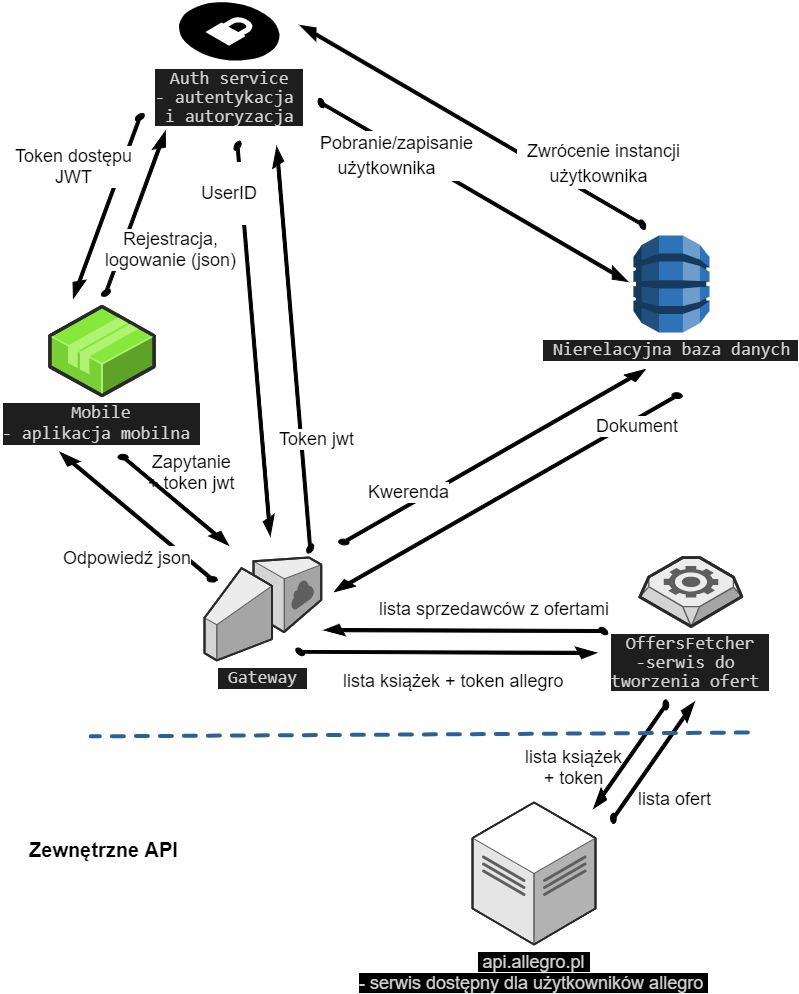
\includegraphics[width=\linewidth]{architecture_overview.png}
	\caption{Struktura systemu}
\end{figure}

\section{Auth service}
Auth service dba o zachowanie bezpieczeństwa w całym systemie.
Poprzez ekstrakcję funkcjonalności związanej z tworzeniem kont, logowaniem oraz zarządzaniem dostępem do pozostałych sektorów, gwarantuje niezawodną autentykację i autoryzację użytkownika pragnącego korzystać z aplikacji.\\
Informacje o kontach użytkowników przechowywane są w bazie danych, do której dostęp uzyskać można tylko za pomocą wygenerowanego przez nią, wewnętrznego klucza. 
\\
W celu swobodnego poruszania się po aplikacji należy uzyskać JWT(\texttt{JSON Web Token}). Aby pozsykać token należy się zarejestrować lub zalogować na ekranie logowania. Zapytanie utworzone w ten sposób zostanie wysłane do Auth service. W odpowiedzi przesłany zostanie wyżej wymieniony klucz dostępowy.\\

\subsection{JSON Web Token}

JSON Web Token to otwarty standard, który definiuje kompaktowy i samodzielny sposób na bezpieczny transfer danych. Poszczególna instancja składa się z trzech części oddzielonych kropkami w bezpośrednim formacie xx..x.y..yy.zz..z, gdzie poszczególne człony reprezentują: \cite{jwt}
\begin{enumerate}%[1)]
	\item Header - nagłówek, zawierający dwie informacje:
		\begin{itemize}
			\item typ tokenu, w tym przypadku "JWT"
			\item algorytm szyfrujący(n.p. HMAC, SHA256 lub RSA)
		\end{itemize}

	\item Payload - lista wyrażeń opisujących szyfrowaną informację, w przypadku użytkownika - np jego login, czy email.
	
	\item Signature - podpis stworzony poprzez zaszyfrowanie podanym w headerze algorytmem szyfrującym ciągu składającego się z
	\begin{itemize}
		\item zakodowanego za pomocą Base64 (specjalnego kodowania transportowego) nagłówka i listy wyrażeń
		\item sekretu, czyli unikalnego dla danych klucza.
	\end{itemize}
	\end{enumerate}

	\begin{figure}[H]
		\centering
		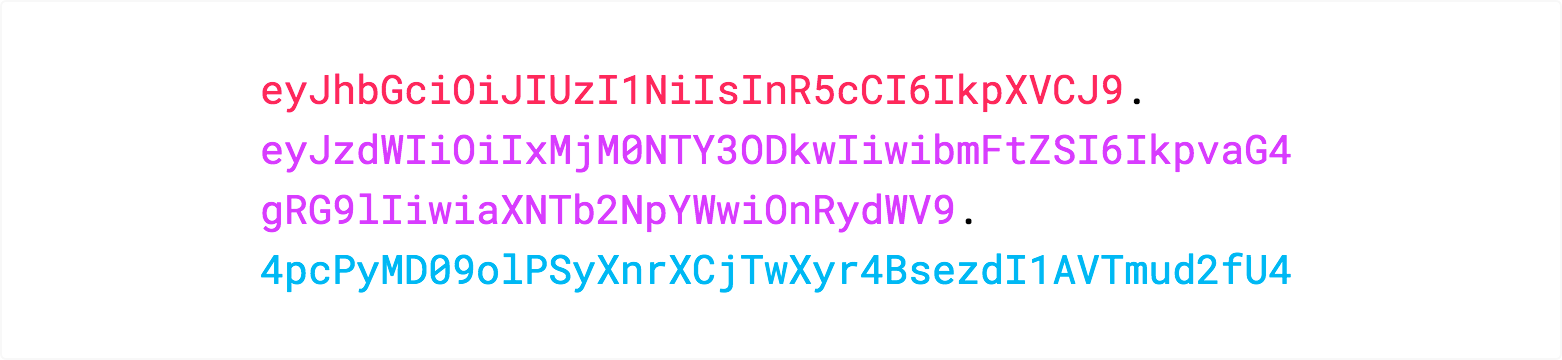
\includegraphics[width=\linewidth]{json-token.png}
		\caption{Przykładowy token jwt \cite{jwt}}
	\end{figure}

\subsection{Autoryzacja, a autentykacja}

Warto implicite rozróżnić dwa bardzo ważne pojęcia związane z bezpieczeństwem aplikacji ze względu na częstotliwość z jaką są one mylone.

\textbf{Autentykacja} - często też w dwóch częściach jako identyfikacja i uwierzytelnienie. Polega na potwierdzeniu tożsamości, to znaczy określeniu, czy podmiot procesu jest tym za kogo się podaje. Na przypadku logowania, strona ufająca otrzymuje od użytkownika podstawue stwierdza, czy użytkownik może być pozytywnie zweryfikowany.

\textbf{Autoryzacja} to potwierdzenie, czy dany użytkownik jest uprawniony do skorzystania z konkretnego zasobu. Na tym etapie autentykacja została ewaluowana pozytywnie. Nie oznacza to jednak, że dany podmiot posiada dostęp w żądanym zakresie. 


\section{Gateway}
Gateway to serwis zbudowany według podejścia zwanego \texttt{wzorcem bramy interfejsu API}\cite{api_gateway}. Jest to element znajdujący się pomiędzy klientem a rozproszonymi usługami. Dzięki temu w prosty sposób można kontrolować wszelkie zapytania skierowane do poszczególnych serwisów.\\
Jest to więc centralny punkt systemu, który ma na celu uproszczenie komunikacji warstwy prezentacyjnej z poszczególnymi usługami. Każde zapytanie wysłane do bramy zostaje zweryfikowane pod względem bezpieczeństwa. Następnie w zależności od potrzeb, modyfikowane, lub bezpośrednio przesłane dalej.
\begin{figure}[H]
	\centering
	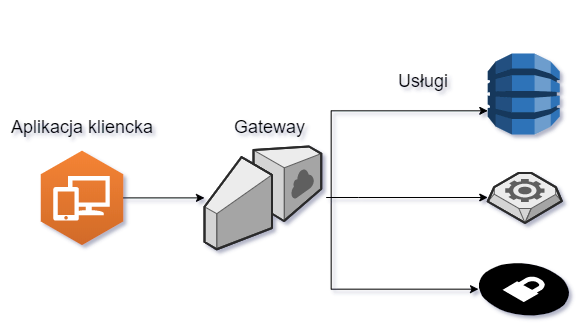
\includegraphics[width=\linewidth]{gateway.png}
	\caption{Gateway - schemat}
\end{figure}

\section{OffersFetcher}
OffersFetcher to główna jednostka licząca w systemie. Usługa ta otrzymuje żądanie z listą książek oraz token dostępowy do REST API portalu Allegro. (3.5.)
Dla każdej książki wykonywane jest odpowiednio zmodyfikowane zapytanie, którego rezultat jest przetwarzany i odkładany do odpowiedniej kolekcji, aby na koniec zostać wkomponowanym w pożądany rezultat. Analizowane są wszystkie obecnie dostępne w czasie rzeczywistym oferty sprzedaży w serwisie Allegro.pl. \\Dane otrzymane w ten sposób są przetwarzane i grupowane po unikalnym identyfikatorze sprzedawcy. Serwis zwraca odpowiedź w postaci listy zbiorów przedmiotów, które wpisują się w pozyzcje otrzymane w zapytaniu. 
\begin{figure}[H]
	\centering
	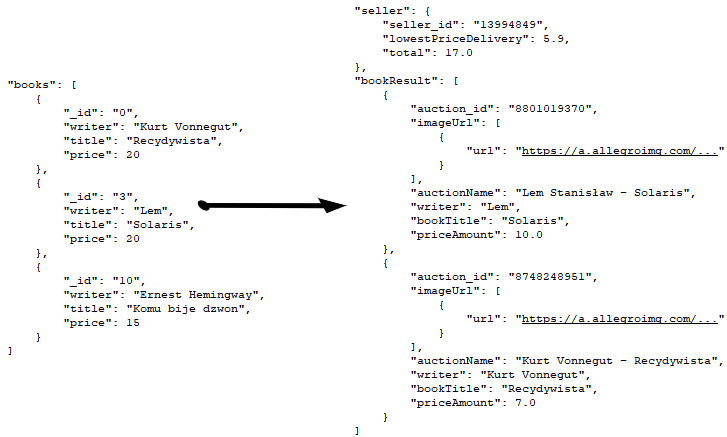
\includegraphics[width=\linewidth]{booksToOffers.png}
	\caption{Poszukiwane książki i bazująca na nich przykładowa oferta}
\end{figure}
\section{Zewnętrzne API}
Źródłem danych dla ofert tworzonych w serwisie OffersFetcher (3.4.)
jest Allegro REST API udostępnione przez Allegro.pl, czyli platformę transakcyjną on-line przedsiębiorstwa Allegro.pl. Portal ten umożliwa użytkownikom wystawianie na sprzedaż posiadanych przez nich przedmiotów oraz na korzystanie z ofert innych sprzedawców.\\
``Allegro REST API działa w oparciu o protokół HTTP (...) Autoryzacja realizowana jest w standardzie OAuth2.``\cite{allegroApi}\\ \newpage
\textbf{REST API} (\textbf{RE}presentational \textbf{S}tate \textbf{T}ransfer) to styl architektury oprogramowania w którym dane i funkcjonalności są odzwierciedlone  poprzez Ujednolicone Identyfikatory Zasobów(w skrócie URI). Termin ten został stworzony przez Roy Fielding w 2000 roku\cite{fielding}.Dostęp uzyskiwany jest poprzez proste i jasno zdefiniowane operacje. \linebreak Istnieje pięc obowiązkowych ograniczeń, które dokładnie definiują charakter tego podejścia:
\begin{itemize}
	\item bezstanowość - każde zapytanie do serwera powinno zawierać wszystkie informacje potrzebne do jego zrozumienia.
	\item użycie buforownia podręcznego - jeżeli dane są lokalnie przechowywane, należy o tym bezpośrednio poinformować.
	\item system warstwowy - istnieje możliwość użycia wielu komponentów do poszczególnych funkcjolności, które razem stanowią jedno API. Klient przeważnie nie jest w stanie określić, czy jego połączenie jest realizowane z serwerem końcowym czy którymś z pośredników.
	\item rozdział klienta od serwera - obie części powinno się być w stanie rozwijać osobno i niezależnie. Klient powinien jedynie znać URI, które może odpytywać.
	\item ujednolicony interfejs - należy deterministycznie zdefiniować i nie zmieniać adresów pod którymi dostępne będą zasoby. 
\end{itemize}
\cite{rest}

\section{Baza danych}
Warstwa persystencyjna jako osobny i niezależny serwis ma zadanie utrzymywać stan aplikacji. Jest to ogromnie ważny element systemu, którego działanie niezbędne jest np dla Auth service(3.2) ze względu na posiadane informacje o użytkownikach, które używane są w celu autoryzacji i autentykacji.
Oprócz danych dostępowych, dla każdego klienta przechowywane są również zbiory książek - posiadanych i poszukiwanych.\linebreak

Bazy danych można podzielić ze wględu na struktruę organizacji danych, którymi się kierują. Są to między innymi  
\section{Aplikacja mobilna}
\chapter{Implementacja}
\label{cha:implementacja}

Ze względu na charakter aplikacji, która składa się z autonomicznych elementów, znaczna część implementacji poszczególnych serwisów mogła odbywać się niezależnie od innych. Tworzone funkcjonalności testowane były przy pomocy narzędzia Postman, za pomocą którego można wysyłać dowolnie skonfigurowane zapytania HTTP na konkretne adresy URI. Kolejne, gotowe usługi były następnie integrowane w sytemie.

%---------------------------------------------------------------------------

\section{Metodyka pracy}
Projekt powstawał iteracyjnie. To znaczy, że podczas pracy zaczynano od małych celów i po ich realizacji - stawiano trochę większe, udoskonalano obecny wówczas stan i przechodzono do kolejnego, bardziej zaawansowanego kroku. W ten sposób, możliwe było dokładne kontrolowanie rozwoju systemu, jego testowanie i w razie problemów, szybka analiza i znalezienie ich przyczyny. 

\subsection{Version Control System}
\textbf{VCS} - postęp prac śledzony był za pomocą systemu kontroli wersji.
Pozwala on dokumentować wszystkie, kolejne zmiany, które mają miejsce w odniesieniu do kodu. Dzięki temu wygodniejsze są również potencjalne eksperymenty, ponieważ w każdym momencie, możliwy jest powrót do dowolnego, poprzedniego stanu implementowanych funkcjonalności.\cite{vcs}\\
W projekcie korzystano z hostingu na platformie GitHub.

\subsection{Organizacja zadań}
\textbf{Kanban} to metodologia, która może być użyta jako narzędzie do zarządania projektem podczas produkcji oprogramowania. Oryginalnie wymyślona w celu optymalizacji produkcji w Japońskiej firmie Toyota. Jej implementacja w procesie rozwijania systemów informatycznych znacząco wzrasta ze względu na przewagę nad tradycyjnymi metodami objawiącej się elastycznością, wydajnością i zwiększoną produktywnością. Sama nazwa oznacza w wolnym tłumaczeniu ``spis widoczny``.\cite{kanban}\\ Głównym elementem jest utworzenie torów, oznaczających poszczególne etapy w których znajdują się obecnie zadania. W momencie zmiany stanu, dany element jest przemieszczany do nastepnej w kolejności kolumny.\\
Korzystając z faktu, że w serwisie Github możliwe jest utworzenie takiej kanbanowej tablicy, zdecydowano się na użycie właśnie tej implementacji narzędzia. Poniżej zaprezentowano stan części planszy podczas rozwoju projektu.
\begin{figure}[H]
	\centering
	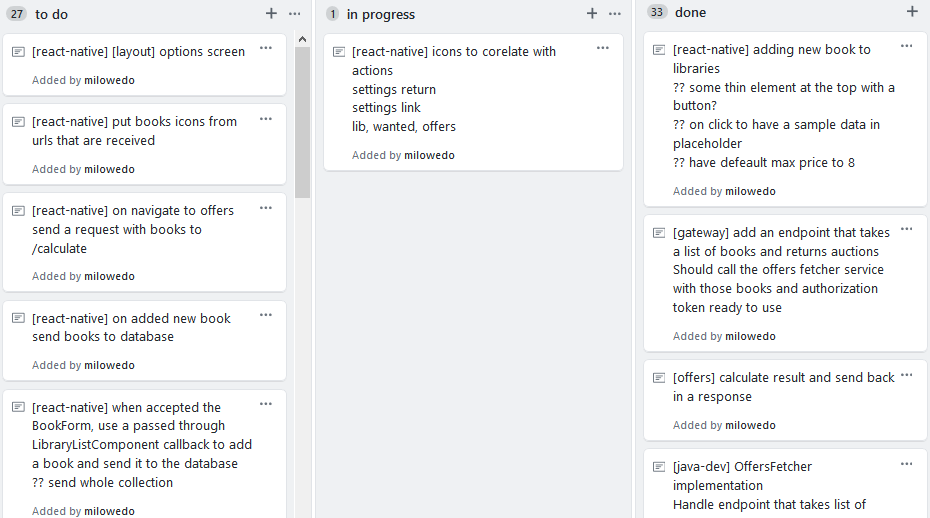
\includegraphics[width=\linewidth]{kanban.png}
	\caption{Kanbanowa tablica podzielona na 3 sektory}
\end{figure}

%---------------------------------------------------------------------------

\section{Wybór technologii}
Językami programowania, które maja największy udział w projekcie są Javascript(2.2, 2.3, 2.7) oraz Java(2.4). Za persystencję odpowiada chmurowa wersja bazy danych NoSQL(2.6.2) - MongoDB Cloud.\\

\subsection{Express}
\textbf{Auth Service} oraz \textbf{Gateway} to serwisy o podobnym stosie technologicznym. Obydwa powstały z pomocą Express js API - javascriptowego frameworku wspierającego implementację serwera obsługującego tworzenie i wystawianie REST API.
\begin{figure}[H]
	\centering
	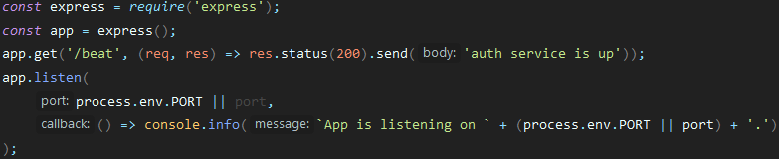
\includegraphics[width=\linewidth]{express_simple.png}
	\caption{Kod odpowiedzialny za wystawienie prostego API}
\end{figure}
Jak przedstawiono powyżej, aby stworzyć nasłuchujący na jednym punkcie końcowym serwer, wystarczy parę linijek kodu. Naturalnie, potrzeby wspomnianych serwisów są większe i potrzebują bardziej zaawansowanego podejścia niż przedstawiono na załączonej grafice.

\subsection{React Native}
\textbf{Aplikacja mobilna} jest napisana na platformie Expo, która jest zestawem narzędzi ułatwiającym prace w stworzonym przez Facebooka frameworku mobilnym - React Native. Został on wybrany, ponieważ jest sprawdzony(Facebook, Instagram, Skype), ciągle udoskonalany i prawdopodobnie nie przestanie być popularny w najbliższym czasie. Posiada on także pokaźną społeczność, co często okazuje się być nieocenionym podczas implementacji.\\
Ciekawym rozwiązaniem zaprezentowanym przez twórców są tak zwane Hooki, które pozwalają używać stanu w wykorzystanych w aplikacji komponentach funkcyjnych - lżejszych niż komponenty klasowe.\\

Przykładem zastosowania jest pobieranie książek (za pomocą funkcji fetchMyBooks()) z bazy danych - wywołanie to potrzebne jest jedynie raz, podczas pierwszego ładowania ekranu MyLibraryScreen. Nie jest pożądanym wysyłać zapytania za każdym razem, kiedy użytkownik powróci do tego samego punktu i tracić zasoby urządzenia - dane są już i tak obecne w pamięci podręcznej. 
\begin{figure}[H]
	\centering
	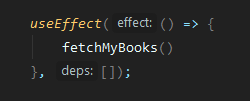
\includegraphics{hook.png}
	\caption{Zastosowanie hooka ``useEffect``}
\end{figure}
Hook \textbf{useEffect} przyjmuje dwa argumenty, pierwszy to funkcja, która ma się wykonać przy inicjalizacji komponentu oraz za każdym razem kiedy element tablicy z drugiego argumentu ulegnie zmianie.

%---------------------------------------------------------------------------

\section{Wielowątkowe tworzenie ofert}
\newpage

%---------------------------------------------------------------------------

\section{Autoryzacja użytkownika w Allegro API}

Do integracji serwisu z aplikacją potrzebne jest pozyskanie tokenu dostępowego. Allegro udostępnia tzw. ``ścieżkę device flow``, dzięki której cały proces odbywa się bez konieczności uwzględniania go w interfejsie graficznym. Poniżej zaprezentowany jest diagram prezentujący tę funkcjonalność.\\

\begin{figure}[H]
	\centering
	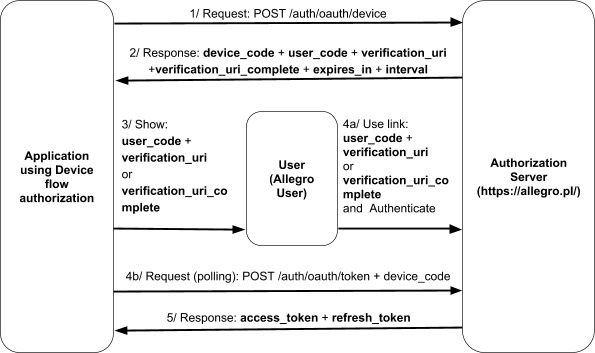
\includegraphics[width=\linewidth]{device_flow.png}
	\caption{Autoryzacja użytkownika typu Device flow}
	\caption*{Źródło: {https://developer.allegro.pl/}}
\end{figure}

Podejście w tej pracy zakłada zarejestrowanie jednego, wspólnego dla całego systemu, konta funkcjonalnego za pomocą którego każde zapytanie będzie autentykowane. Stwarza to niestety jedno ograniczenie, a mianowicie, ze względu na obowiązujący główny limit nakładany na Client ID po przekroczeniu liczby 9000 zapytań na minutę, aplikacja zwróci status HTTP 429 i zostanie zabklokowana na kolejne 60 sekund.\\
W fazie inicjalizacyjnej autoryzacji uzyskane zostaną dwa unikalne tokeny: 
\begin{itemize}
	\item dostępowy - ważny przez 12h.
	\item odświeżający - ważny 6 miesięcy.
\end{itemize}
Zostaną one zachowanie w pamięci, a każde kolejne zapytanie, w przypadku wygaśnięcia tokenu dostępowego, spowoduje jego odnowienie.
\begin{figure}[H]
	\centering
	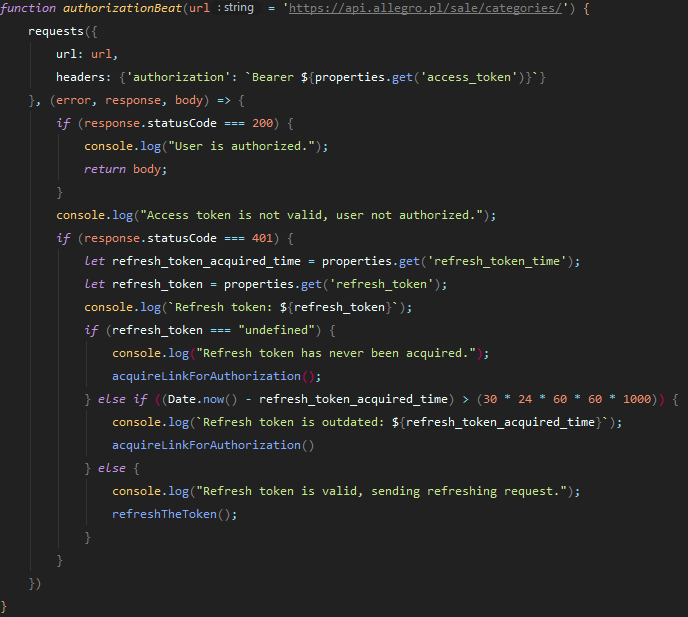
\includegraphics[width=\linewidth]{authorization.png}
	\caption{Kod odpowiedzialny za utrzymywanie ważnego tokena}
\end{figure}
Powyższy kod prezentuje przebieg akcji, które maja miejsce za każdym razem, kiedy otrzymywane jest zapytanie do OffersService(2.4). Na początku sprawdzane jest, czy token jest zwyczajnie aktualny, następnie, w przypadku, gdy nie jest, pobierany jest token odświeżający. W zależności od tego, czy jest on ważny, wygaśnięty, czy może w ogóle nigdy nie został uzyskany, odpowiednia logika zostaje uruchomiona.

%---------------------------------------------------------------------------

\section{MongoDB Cloud}
 
Modele przechowujące dane są zdefiniowane w klasach User.js i
oraz Book.js. Połączenie do bazy danych jest obsłużone przy pomocy bilbioteki ``mongoose``. Potrzebny jest jedynie tak zwany connection string, który uzyskany został poprzez zalogowanie się na stronie webowej serwisu hostującego cloud.mongodb.com i nawigację do zakładki Connect.\\
\begin{figure}[H]
	\centering
	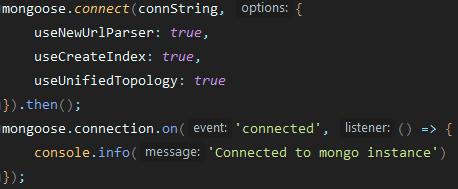
\includegraphics[width=\linewidth]{mongo.png}
	\caption{Połączenie do bazy danych MongoDB}
\end{figure}
W załączonej grafice widać rozpoczęcie połączenia z bazą danych. Ważnym elementem jest opcja \textbf{useCreateIndex}, dzięki której znajdujące się w serwisach Auth Service i Gateway, modele, otrzymają indeksy pod którymi znaleźć będzie można zapisane dokumenty. 

%---------------------------------------------------------------------------

\section{Wdrożenie}

Korzystanie ze stworzonych serwisów jest umożliwione poprzez wdrożenie ich na platformie chmurowej Heroku.
W ten sposób każda usługa posiada własne URI, na które wysyłane są zapytania w zależności od potrzeb.
Poszczególne aplikacje możnaby również uruchomić na pojedynczym komputerze, jednakże wymagałoby to sporej ilości zasobów, stąd zdecydowano się na rozwiązanie hostingowe.\\

Minimalne środowisko jakie jest wymagane aby uruchomić system to:
\begin{itemize}
	\item Node v10.13.0
	\item Java v11
	\item Maven v3.5
	\item Gradle v6.0
	\item Expo v3.11.1
\end{itemize}

Wdrożenie wymagało stworzenia aplikacji w sensie logicznym za pomocą lini komend Heroku CLI oraz wskazania adresu URI do stosownych repozytoriów Github, gdzie przetrzymywany jest kod.
W ten sposób w webowym interfejsie pod adresem dashboard.heroku.com znalazły się odnośniki reprezentujące trzy usługi : OffersFetcher, Auth Service oraz Gateway. Każda z nich ma zdefiniowaną odpowiednią konfigurację, dzięki której aplikacje mogą zostać uruchomione.
\begin{itemize}
	\item {OffersFetcher uruchamiany jest na platformie poleceniem \textit{web java -jar build/libs/*.jar}}
	\item {AuthService oraz Gateway - komendą \textit{npm start}}
\end{itemize}

Aby uruchomić lokalnie aplikację mobilną należy w folderze ją zawierającym wykonać polecenie \textit{expo r}.

%---------------------------------------------------------------------------
\chapter{Interfejs}
\label{cha:interfejs}

Interfejs aplikacji składa się z trzech rodzielnych zbiorów ekranów. Każda nawigacja pomiędzy tymi grupami skutkuje usunięciem z pamięci kolekcji ekranów, znajdujących się w poprzedniej grupie oraz załadowaniem nowego zestawu.
W pierwszym pakiecie znajdują ekrany logowania i rejestracji. Jeżeli użytkownik zaloguje się lub zarejestruje, jego token dostępowy zostanie zapisany w pamięci podręcznej urządzenia i do momentu jej wyczyszczenia, program nie będzie wymagał od niego ponownego wpisywania swoich danych w celu autoryzacji. Co za tym idzie, w ogóle nie zaistnieje potrzeba załadowania tych widoków.
Po autoryzacji użytkownik otrzymuje dostęp do drugiego i trzeciego zbioru zawierających :
\begin{enumerate}
    \setcounter{enumi}{1}
    \item dwie biblioteki oraz widok z zaprezentowanymi ofertami
    \item ustawienia
\end{enumerate} 

\begin{figure}[H]
	\centering
	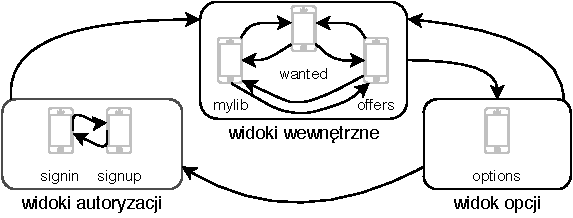
\includegraphics[width=\linewidth]{navig.pdf}
	\caption{\centering Schemat nawigacji pomiędzy ekranami}
	\caption*{\centering Źródło: {Opracowanie własne za pomocą narzędzia \url{https://www.draw.io/}}}
\end{figure}
%---------------------------------------------------------------------------

\section{Logowanie i rejestracja}
Te dwa ekrany zawierają formularze w których użytkownik może wpisać email oraz hasło. Po wpisaniu danych, akceptuje formularz niebieskim przyciskiem i tworzy zapytanie do Auth Service. W sytuacji, gdy wprowadzone dane są niewłaściwe, zostanie wyświetlony odpowiedni komunikat.
Na dole ekranu widnieje krótki tekst, po którego kliknięciu, nastąpi zresetowanie formularza i przeniesienie do sąsiedniego widoku.

\begin{figure}[H]
	\centering
	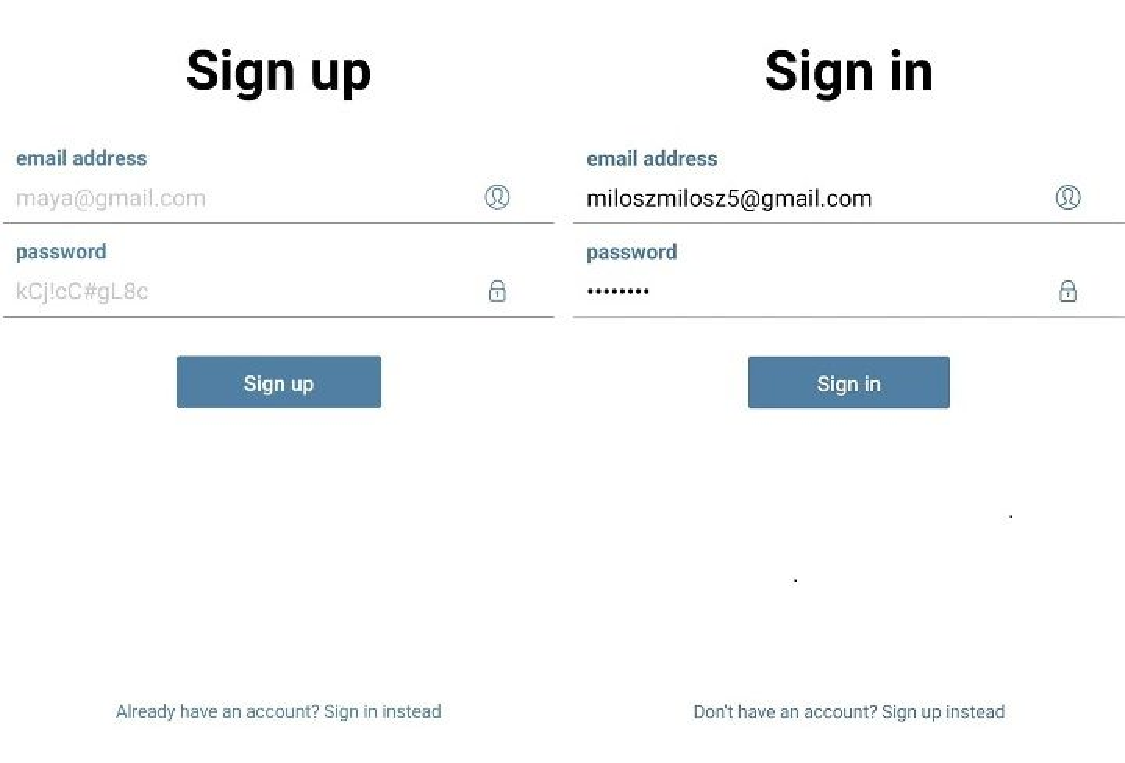
\includegraphics[width=\linewidth]{signin_signup.pdf}
	\caption{\centering Ekrany logowania i rejestracji w aplikacji mobilnej}
	\caption*{\centering Źródło: {Opracowanie własne}}
\end{figure}
%---------------------------------------------------------------------------
\section{Ekrany bibliotek}
Widoki \textit{Wanted} i \textit{My library} korzystają w większości z tych samych komponentów, różni je natomiast sposób oraz cel ich użycia. Obydwa zawierają listy(rodzaj komponentu), których jedynie widoczne elementy są renderowane, aby nie spowalniać pracy aplikacji. Można je przesuwać werykalnie, a każdy element posiada ukryte opcje z lewej i prawej strony, które można aktywować poprzez horyzontalne przesunięcie wykonane na pojedynczym segmencie.


Widok poszukiwanych książek prezentuje pozycje, które będą wysłane do serwisu OffersFetcher  i użyte w celu stworzenia ofert.
Na poniższej grafice widnieje funkcjonalność dodawania nowej pozycji do listy. Po naciśnięciu  obszaru z napisem ``new book``, wysunięty zostanie formularz, który poprawnie wypełniony poskutkuje dodaniem nowej książki i wysłaniem jej do bazy danych w chmurze. Cenę każdej pozycji można edytować po jej naciśnięciu - pojawi się pole do edytowania wartości.
\begin{figure}[H]
	\centering
	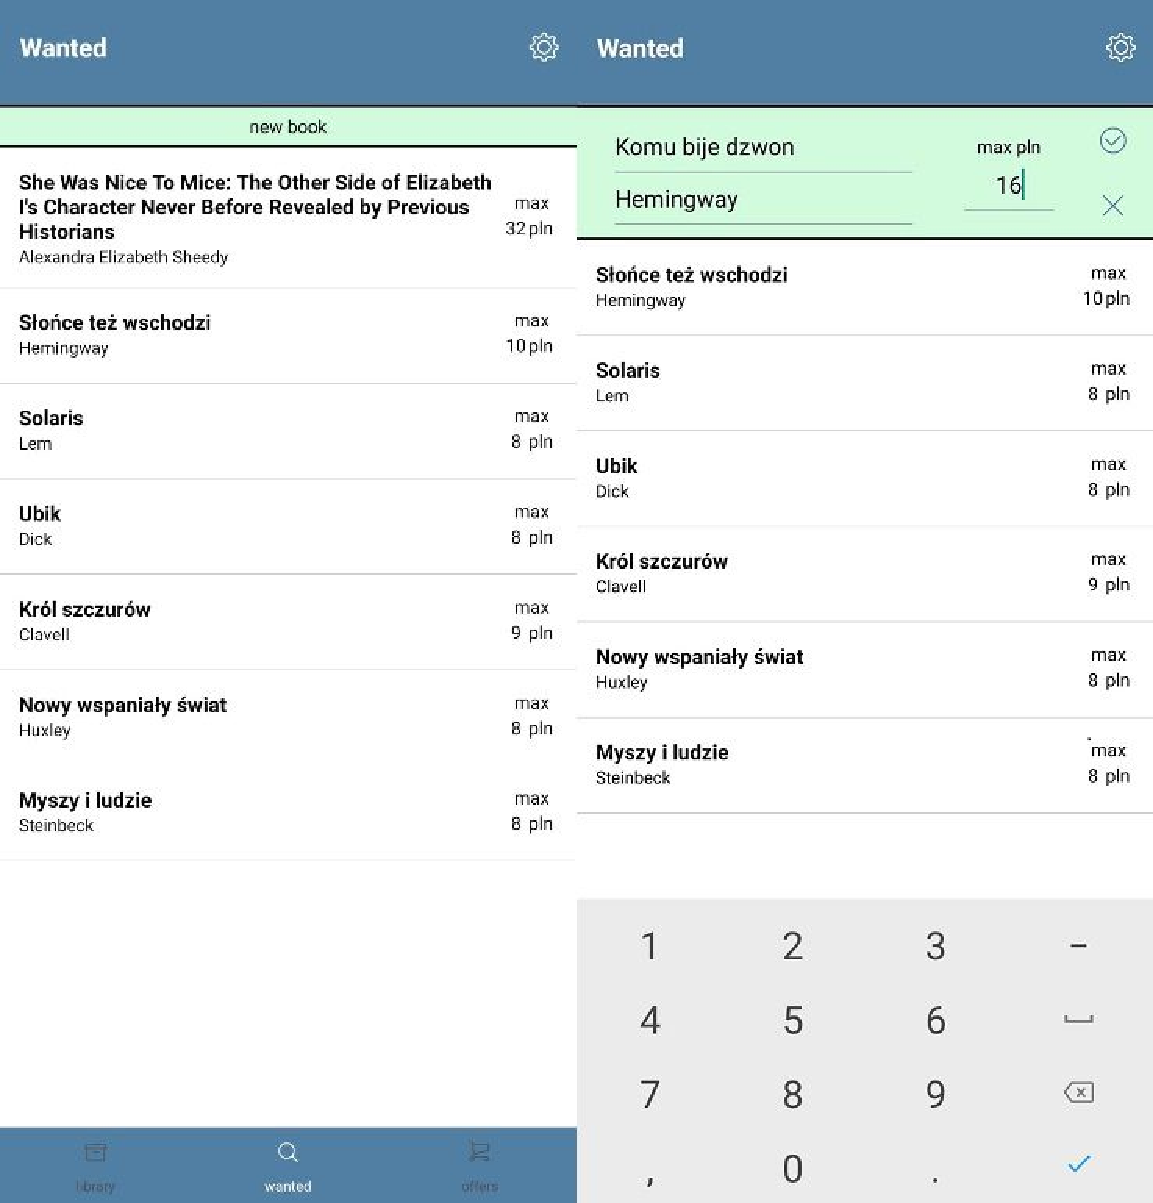
\includegraphics[width=\linewidth]{wanted.pdf}
	\caption{\centering Biblioteka poszukiwanych książek oraz dodawanie nowej pozycji}
	\caption*{\centering Źródło: {Opracowanie własne}}
\end{figure}


Poprzez przesunięcie pojedynczego elementu w lewo, pojawi się ukryty pod spodem przycisk, który służy do usunięcia danej książki z listy i bazy danych. Jeżeli bloczek poruszony zostanie ruchem o przeciwnym zwrocie, użytkownik otrzyma możliwość edytowania informacji o danym tomie.
Każde wychylenie elementu zostanie przywrócone do stanu wyjściowego w momencie poruszenia innej pozycji lub po 5 sekundach bezczynności.
\begin{figure}[H]
	\centering
	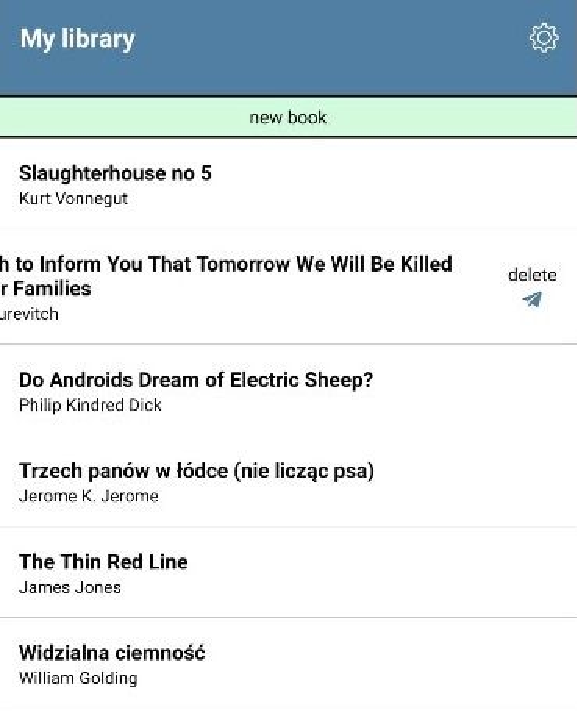
\includegraphics{mylib.pdf}
	\caption{\centering Bilbioteka posiadanych książek oraz funkcjonalność usuwania}
	\caption*{\centering Źródło: {Opracowanie własne}}
\end{figure}

%---------------------------------------------------------------------------

\section{Ekran z ofertami}
To tutaj zaprezentowane są wyniki analiz wykonanych w serwisie OffersFetcher. Jest to przesuwalny wertykalnie komponent zawierający sprzedawców oraz ich produkty, na bazie pozycji z ekranu Wanted. Każdy element składa się z identyfikatora właściciela aukcji, następnie z listy książek, gdzie każdy obiekt to zdjęcie prezentujące produkt, tytuł, autor, a także jego cenę. Na dole oferty wyświetlona jest sumaryczna cena tomów oraz najtańsza możliwa dostawa według kontrahenta.
\begin{figure}[H]
	\centering
	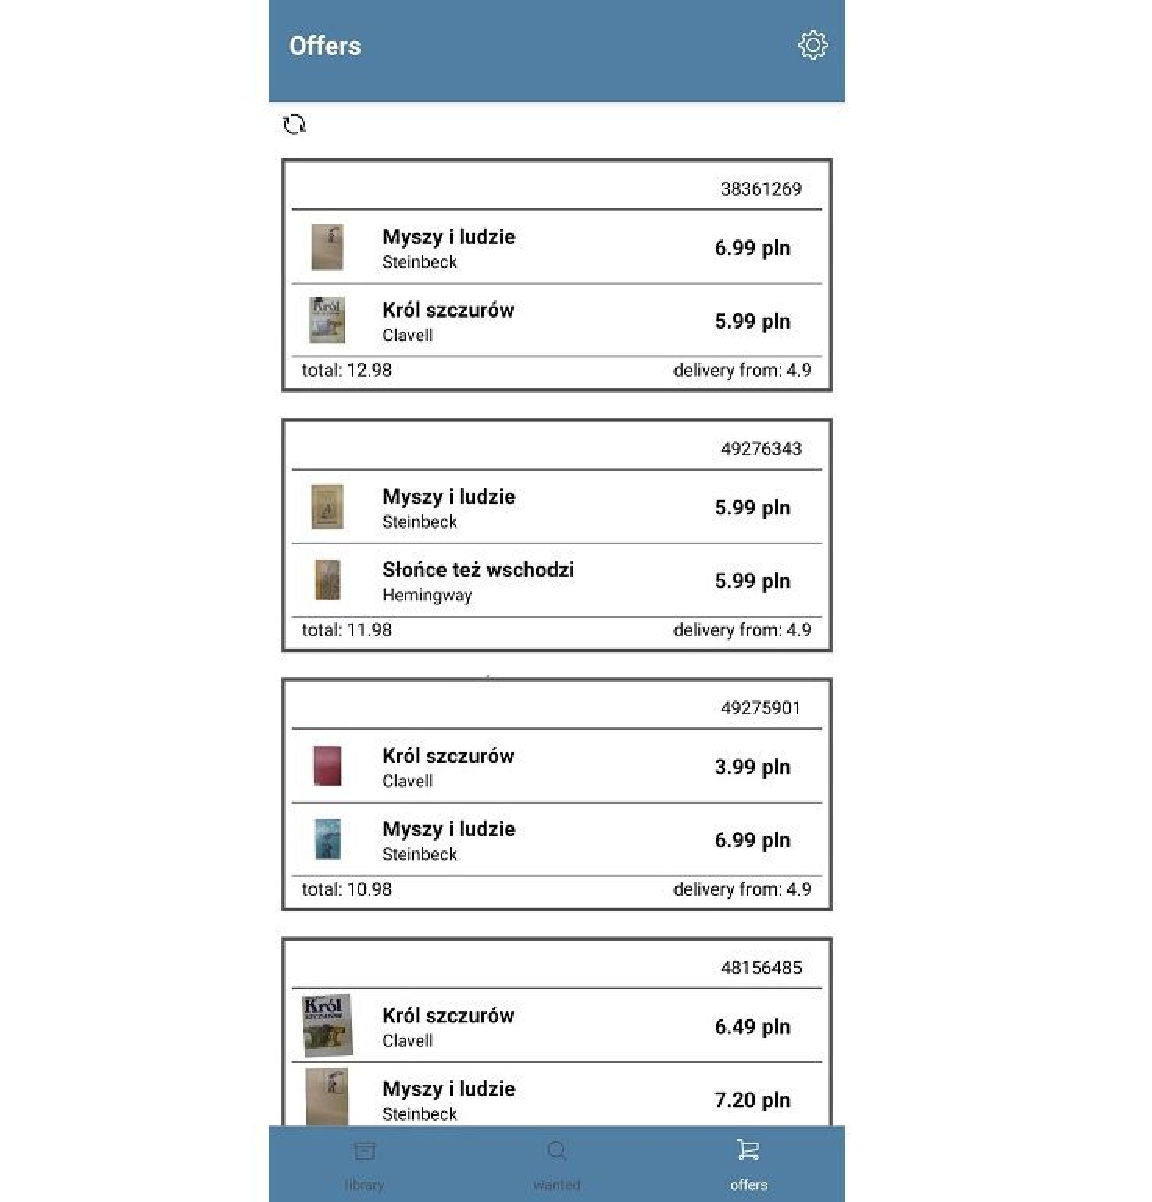
\includegraphics[width=\linewidth]{offers.pdf}
	\caption{\centering Ekran prezentujący oferty od sprzedawców}
	\caption*{\centering Źródło: {Opracowanie własne}}
\end{figure}

\newpage
\section{Opcje}
Obecnie na ekranie opcji, który można wywołać po naciśnięciu przycisku w prawym górnym rogu, dostępna jest tylko jedna opcja - mianowicie wylogowanie użytkownika. Po naciśnięciu przycisku, usunięty zostanie token dostępowy, a aplikacja wykona przeniesienie do ekranu logowania.
\begin{figure}[H]
	\centering
	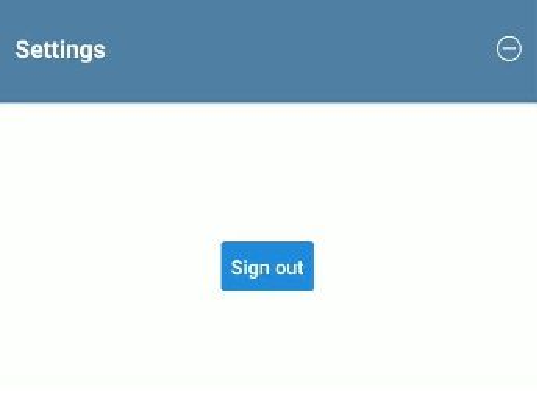
\includegraphics{options.pdf}
	\caption{\centering Ekran opcji z możliwością wylogowania}
	\caption*{\centering Źródło: {Opracowanie własne}}
\end{figure}


\chapter{Podsumowanie}
\label{cha:podsumowanie}

Projekt i implementacja przedstawionego w tej pracy systemu zostały wykonane\\w sposób wystarczająco zadowalający. Użytkownik może w zaledwie parę sekund otrzymać wyniki przeanalizowania setki możliwych ofert od sprzedawców na platformie Allegro.pl. Aplikacja jest w stanie przetrzymywać listy książek dla użytkowników w zewnętrznym, zabezpieczonym przed nieautoryzowanym dostępem, archiwum chmurowym. Brak więc obaw o utratę danych z urządzenia mobilnego. Czasochłonne obliczenia i analizy dostępnych w serwisie aukcyjnym przedmiotów wyekstraktowano do osobnego serwisu\\o zdecydowanie większej mocy obliczeniowej niż przeciętny komputer podręczny.
%---------------------------------------------------------------------------

\section{Wnioski}
W procesie tworzenia aplikacji dzięki podjętym decyzjom i rozwiązanym problemom, autorowi tej pracy udało się nabyć cenne doświadczenie. 
Użycie nierelacyjnej bazy danych można określić jako rozwiązanie trafne i wydajne. Również integracja z zewnętrznym API platformy Allegro.pl jest najtrafniejszą decyzją, jaką autor mógł podjąć, decydując się na źródło danych dla aplikacji.\newline
Sporym wyzwaniem było na pewno połączenie poszczególnych serwisów wdrożonych jako osobne aplikacje w jeden, komunikujący się między sobą twór.\newline
System jest zabezpieczony przed nieautoryzowanym dostępem. Jego budowa to luźno powiązane elementy, które można odłączać i modyfikować bez destrukcyjnego wpływu na działanie całości aplikacji.
W łatwy sposób można ją rozszerzyć, dodając kolejne serwisy i włączając je w odpowiednich miejscach.

\newpage
\section{Możliwe rozszerzenia i usprawnienia}
Przygotowany system jest dobrze przygotowany na przyjęcie kolejnych ulepszeń i możliwości.\newline
Zdecydowanie ciekawym usprawnieniem byłaby na przykład możliwość łączenia baz poszukiwanych książek z bilbiotekami innych użytkowników, czy większa personalizacja wyszukiwań pod kątem chociażby czasowego wykluczania niektórych pozycji z analizy.\newline
Bazując również na posiadanych tomach, warte byłoby rozważenie algorytmów, które potrafiłyby wskazać użytkownikowi rekomendowane przez system pozycje o których sam nie pomyślał.
Z uwagi na to, że struktura systemu składa się z osobnych serwisów, w łatwy sposób można zaadaptować dowoloną ilość nowych funkcjonalności. Stworzona w poniższej pracy aplikacja ma spory potencjał na rozwój.



% itd.
% \appendix
% \include{dodatekA}
% \include{dodatekB}
% itd.

\printbibliography

\end{document}
